\begin{frame}{Introduction to data assimilation}
    Data assimilation is widely used in:
    \begin{enumerate}[\textbullet]
           \item weather forecasting
           \item ocean simulation
    \end{enumerate}	 
          The main idea of computational data assimilation is to combine:
    \begin{enumerate}[\textbullet]
           \item a model
           \item some observations
    \end{enumerate}	 
    The best estimation:
    $$x^a=Lx^b+Ky^0$$
    with $x^a$ the analyzed state, $x^b$ the state of the model and $y^0$ the observations.
   \end{frame}

   \subsection{Theory}
   
   \begin{frame}[allowframebreaks]{Statistical approach : Derivation of the Kalman filter}
       The Kalman filter method consists in looking for $x^a$ as linear combination of our model and our observations.
       \begin{equation*}
           x^a=x^b+K(y-x^b)
           \label{eq1}
       \end{equation*}
       with K the gain matrix.
    \newpage
        The Kalman filter method consists in looking for $x^a$ as linear combination of our model and our observations.
       \begin{equation}
           x^a=x^b+K(y-x^b)
           \label{eq1}
       \end{equation}
       with K the gain matrix.
       \newline Let’s consider that true state $x^t$ exists:
       \begin{equation}
           x^a-x^t=x^b-x^t+K(y-x^t-x^b+x^t)
       \end{equation}
       Errors: \qquad $\epsilon^a=x^a-x^t,\qquad \epsilon^b=x^b-x^t, \qquad \epsilon^y=y-x^t$ \\
       One realisation of these errors :$ \quad \epsilon^a=\epsilon^b+K(\epsilon^y-\epsilon^b)$ \\
       Many realisation of these errors + sample average :
       \begin{equation}
           <\epsilon^a>=<\epsilon^b>+K(<\epsilon^y>-<\epsilon^b>)
       \end{equation}
    \end{frame}
    \begin{frame}{Kalman filter in one-dimension}

       Analysis error variance as low as possible.
       \newline Minimize $<(\epsilon^a)^2>$ with respect to $K$ :
       $$<(\epsilon^a)^2>=<(\epsilon^b)^2>+K^2<(\epsilon^y-\epsilon^b)^2>+2K<\epsilon^b(\epsilon^y-\epsilon^b)^2>$$
       The errors in the background and observation are uncorrelated.
       $$K=\frac{<(\epsilon^b)^2>}{<(\epsilon^b)^2>+<(\epsilon^y)^2>} \Rightarrow K=\frac{(\sigma^b)^2}{(\sigma^b)^2+(\sigma^y)^2} $$
       $(\sigma^y)^2$ the observation error variance, \newline $(\sigma^b)^2$ the background or model error variance.
   
	\end{frame}
       
	\begin{frame}{Kalman filter in multi-dimensional case}
       Now that we have explained the method for finding $x^a$ let's try to generalize our formula in a \textbf{multi-dimensional case}.
   
       $$\left\{\begin{aligned}
	     &x^a=(I-KH)x^b+Ky^0=x^b+K(y^0-H(x^b)) \\
	           &K=BH^T(HBH^T+R)^{-1} \\
	    \end{aligned}\right.$$
       With $K$ the gain or weight matrix.
       The Best Linear Unbiased Estimator (BLUE).
       \begin{figure}[H]
           \pgfimage[width=0.4\linewidth]{images/enkf/schema_kalman_filter.png}
           \caption{Kalman Filter}
       \end{figure}
   \end{frame}
   \begin{frame}{3D Var : Minimizing a cost function}
       Solves the analysis problem through an optimisation (minimisation of a cost-function)
       Variational approach of BLUE consists in finding $x^a=\arg\min_{x}J$:
       $$\begin{aligned}
           J(x)&=\frac{1}{2}(x^b-x)^TB^{-1}(x^b-x)+\frac{1}{2}(y-H(x))^TR^{-1}(y-H(x)) \\
           &=\frac{1}{2}\|x-x^b\|_B^2+\frac{1}{2}\|H(x)-y^0\|_R^2
       \end{aligned}$$
       \begin{figure}
           \centering
           \pgfimage[width=0.5\linewidth]{images/enkf/schema_3D_Var.png}
           \caption{3D-Var}
       \end{figure}
   \end{frame}
   \begin{frame}{Ensemble Kalman Filter}
       The ENKF method consists in using the Kalman filter in non-linear system.
       \newline We apply the Kalman filter on several state samples $x_1,x_2,..,x_{m}$.
       $$x_i^a=x_i^f+K[y-h(x_i^f)]$$
       with $h(x_i^f)$ the observation operator.
       We can also define the Kalman gains: 
       $$K=P^f H^T(HP^f H^T+R)^{-1}$$
       For exemple we can estimate the
       forecast error covariance matrix as:
       $$P^f=\frac{1}{m-1}\sum_{i=1}^{m}(x_i^f-\bar{x}^f)(x_i^f-\bar{x}^f)^T~~\text{with}~~\bar{x}^f=\frac{1}{m}\sum_{i=1}^{m}x_i^f $$ .
   \end{frame}

   \subsection{Results}

   \begin{frame}{Harmonic oscillator}
       \small
       $(x(0),v(0))=(2,0)$, \quad $Pe$=$\frac{2\pi}{\omega_0}$, \quad $\omega_0=2$, \quad $x_0=2$ \quad, $\phi_0=0$ \quad $dt$=$\frac{Pe}{20}$, \quad $[t_0,T]=[0,3Pe]$
       \begin{minipage}{.32\linewidth}
           \centering
           $$P=\begin{pmatrix}
               0.01 & 0. \\ 
               0. & 0.01 
           \end{pmatrix} ,$$
           $$Q=\begin{pmatrix}
               0.01 & 0. \\
               0. & 0.01 
           \end{pmatrix} ,$$
           $$R=0.001$$
           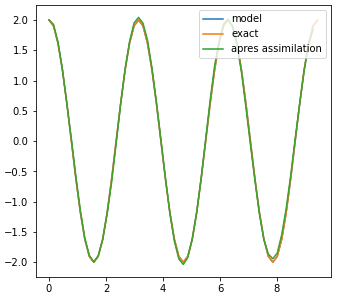
\includegraphics[width=\linewidth]{"images/enkf/oscillator1_b.png"}
       \end{minipage} \;
       \begin{minipage}{.32\linewidth}
           \centering
           $$P=\begin{pmatrix}
               1. & 0. \\
               0. & 1. 
           \end{pmatrix} ,$$
           $$Q=\begin{pmatrix}
               0.01 & 0. \\
               0. & 0.01 
           \end{pmatrix} ,$$
           $$R=0.001$$
           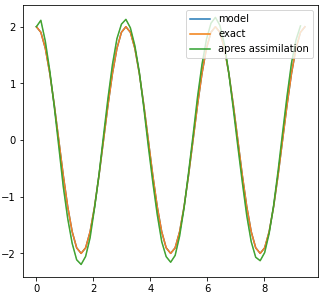
\includegraphics[width=\linewidth]{"images/enkf/oscillator2_b.png"}
       \end{minipage} \;
       \begin{minipage}{.32\linewidth}
           \centering
           $$P=\begin{pmatrix}
               0. & 0. \\
               0. & 0. 
           \end{pmatrix} ,$$
           $$Q=\begin{pmatrix}
               0. & 0. \\
               0. & 0. 
           \end{pmatrix} ,$$
           $$R=0.001$$
           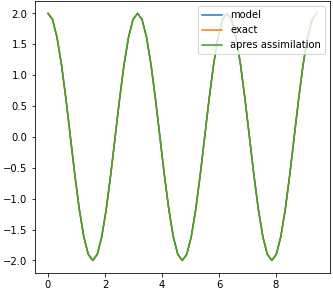
\includegraphics[width=\linewidth]{"images/enkf/oscillator3_b.png"}
       \end{minipage}
       
   \end{frame}
   \begin{frame}{Lorenz System - Same parameters}
    \begin{enumerate}[\textbullet]
        \item $(\sigma, r, b)=(12.,6.,12.)$, $\quad X_0=(-10.,-10.,25.)$, $\quad [t_0,T]=[0,1]$,
        \item We trust much more the observation
        \end{enumerate}
        $$P=\begin{pmatrix}
        0.1 & 0. & 0. \\
        0. & 0.1 & 0. \\
        0. & 0. & 0.1 \\
        \end{pmatrix}, \qquad
        Q=\begin{pmatrix}
        0.1 & 0. & 0. \\
        0. & 0.1 & 0. \\
        0. & 0. & 0.1 \\
        \end{pmatrix},\qquad
       	R=\begin{pmatrix}
        0.01 & 0. & 0. \\
        0. & 0.01 & 0. \\
        0. & 0. & 0.01 \\
        \end{pmatrix}.$$
        \pgfimage[width=1.002\linewidth]{images/enkf/lorenz_1.png}
    \end{frame}
	\begin{frame}[allowframebreaks]{Lorenz System - Differents parameters}
       
       \begin{enumerate}[\textbullet]
           \item Model $(\sigma, r, b)=(10.,6.,10.)$, Observation $(\sigma, r, b)=(12.,6.,12.)$,
           \item $X_0=(-10.,-10.,25.)$, $\quad \Delta t=0.1s$ $\quad [t_0,T]=[0,4]$,
           \item We trust much more the model .
           \end{enumerate}
       		\footnotesize
           $$P=\begin{pmatrix}
           0.1 & 0. & 0. \\
            0. & 0.1 & 0. \\
           0. & 0. & 0.1 \\
           \end{pmatrix},\qquad
           Q=\begin{pmatrix}
            0.01 & 0. & 0. \\
           0. & 0.01 & 0. \\
           0. & 0. & 0.01 \\
           \end{pmatrix}, \qquad 
           R=\begin{pmatrix}
           0.1 & 0. & 0. \\
           0. & 0.1 & 0. \\
           0. & 0. & 0.1 \\
           \end{pmatrix}.$$
   			\normalsize
       \begin{figure}
           \centering
           \pgfimage[width=0.87\linewidth]{images/enkf/lorenz_2.png}
       \end{figure}
   
       \newpage
    
       \begin{enumerate}[\textbullet]
                \item Model $(\sigma, r, b)=(10.,6.,10.)$,Observation $(\sigma, r, b)=(12.,6.,12.)$,
               \item $X_0=(-10.,-10.,25.)$, $\quad \Delta t=0.1s$ $\quad [t_0,T]=[0,4]$,
               \item We trust much more the observation .
            \end{enumerate}
        \footnotesize
            $$P=\begin{pmatrix}
            0.1 & 0. & 0. \\
             0. & 0.1 & 0. \\
            0. & 0. & 0.1 \\
            \end{pmatrix},\qquad
       		Q=\begin{pmatrix}
             0.1 & 0. & 0. \\
            0. & 0.1 & 0. \\
            0. & 0. & 0.1 \\
            \end{pmatrix}, \qquad
            R=\begin{pmatrix}
            0.01 & 0. & 0. \\
            0. & 0.01 & 0. \\
            0. & 0. & 0.01 \\
            \end{pmatrix}.$$
   		\normalsize
       \begin{figure}
           \centering
           \pgfimage[width=0.89\linewidth]{images/enkf/lorenz3_b.png} 
       \end{figure}
   \end{frame}
       